\section{Οικογένειες Αθροιστών}
Στο προηγούμενο κεφάλαιο περιγράφηκε ένας απλός σχεδιασμός αθροιστή. Σε αυτή την ενότητα θα πραγματοποιηθεί η κατάταξη αυτού του αθροιστή σε μία κατηγορία, καθώς και η παρουσίαση μερικών ακόμα βασικών αρχιτεκτονικών. Επίσης θα αποδοθεί μια σύντομη περιγραφή, αναφέροντας πλεονεκτήματα και μειονεκτήματα για κάθε δομή. 



\subsection{Διάδοσης Κρατουμένου}
Αθροιστής Διάδοσης Κρατουμένου ή Ripple-Carry Adder (RCA) είναι ο πιο απλός αθροιστής και το σχηματικό του παρουσιάστηκε στην εικόνα \ref{IntegerAdderSchematic}. Παρατηρείται πως για να υπολογιστεί το $sum_1$ δηλαδή το δεύτερο λιγότερο σημαντικό ψηφίο του αθροίσματος πρέπει πρώτα να υπολογιστεί το $c_{out}$ του προηγούμενου πλήρη αθροιστή, δηλαδή το $c_0$. Αντίστοιχα για το τρίτο πρέπει να υπολογιστεί πρώτα το $c_0$ έπειτα από τον δεύτερο πλήρη αθροιστή να υπολογιστεί το $c_1$ με είσοδο το $c_0$ του προηγούμενου FA. Επομένως κάθε FA δεν λειτουργεί παράλληλα με τα υπόλοιπα στοιχεία άθροισης, αλλά υπάρχει μια χρονική καθυστέρηση για να λάβει την σωστή είσοδο $c_{in}$. Αποτέλεσμα αυτού είναι πως στην χειρότερη περίπτωση, δηλαδή στην περίπτωση που το $c_{in}$ επηρεάζει άμεσα την τιμή του $c_{out}$ του αθροιστή, υπάρχει γραμμική αύξηση της καθυστέρησης με το μήκος του.
Για παράδειγμα έχοντας έναν δυαδικό αθροιστή 8 ψηφίων και εισάγοντας τους αριθμούς Α = 00000000 και Β = 11111111 και $c_{in}$ = 0 θα πάρουμε έξοδο sum = 11111111 και $c_{out}$ = 0 . Αν κρατώντας όλες τις εισόδους σταθερές και αλλάζοντας μόνο την Α σε 00000001 δηλαδή το $A_0$=1 τότε το αποτέλεσμα θα είναι sum=00000000 και $c_{out}$ = 1. 

Η περίπτωση που περιγράφηκε ανήκει στις χειρότερες περιπτώσεις διότι μία αλλαγή στο λιγότερο σημαντικό ψηφίο για να διαδοθεί στο σημαντικότερο ψηφίο του αθροίσματος καθώς και στο τελικό κρατούμενο εξόδου του αθροιστή, πρέπει να περάσει από όλα τα ενδιάμεσα στοιχεία άθροισης. Αυτό συνεπάγει και την άθροιση των καθυστερήσεων του κάθε FA στοιχείου. Παρόμοια περίπτωση θα καταγράφονταν αν άλλαζε η τιμή του κρατουμένου εισόδου, από μηδέν σε ένα, αντί του αριθμού A.


\subsection{Παράλειψής Κρατουμένου}
Για κάθε ψηφίο του αριθμού Α και Β ορίζονται δυο ακόμα στοιχεία , αυτά που παράγουν κρατούμενο ανεξάρτητα του κρατουμένου εισόδου του αντίστοιχου FA και θα καλούνται generate και αυτά που διαδίδουν κρατούμενο και ονομάζουμε propagate. Σημειώνεται πως τα σήματα generate και propagate αναφέροντε στα ζεύγη των δυαδικών ψηφίων των αριθμών εισόδου, δηλαδή $(A_i,B_i)$. Οι εξισώσεις είναι αντίστοιχα :
\begin{equation}
\begin{split}
    g_i &= A_i * B_i  \\
    p_i &= A_i \oplus B_i 
\end{split}
\end{equation}
ή
\begin{equation*}
    p_i = A_i + B_i
\end{equation*}
Όταν ισχύει $g_i=1$ τότε γνωστοποιείται πως ο συγκεκριμένος πλήρης αθροιστής παράγει κρατούμενο εξόδου ανεξάρτητα του κρατουμένου εισόδου. Σε αντίθεση με την συνάρτηση εξόδου του $c_{out}$ του Full-Adder η συνάρτηση του generate είναι πιο απλή καθώς αποτελείται από μόνο μια πύλη AND άλλα δεν εγγυάται την ύπαρξη κρατούμενο εισόδου. Δηλαδή αν $g_i=1$ τότε και $c\_out_i=1$ χωρίς να ισχύει το αντίθετο. 

%-----------------
Οι αθροιστές Παράλειψής Κρατουμένου ή Carry Skip είναι μια υλοποίηση που βελτιώνει την καθυστέρηση διάδοσης κρατουμένου με έναν απλό τρόπο αλλά όχι αρκετά αποτελεσματικό σε σχέση με άλλες αρχιτεκτονικές. 
Η χείριστη περίπτωση παρουσιάζεται παρομοίως με έναν ripple-carry, όταν το propagate στοιχείο είναι αληθές για κάθε ζευγάρι ψηφίων $(A_i B_i)$.
Ορίζοντας τον propagate όρο ως το XOR των $Α_i B_i$, όταν όλοι οι όροι propagate είναι αληθείς τότε το κρατούμενο εισόδου προσδιορίζει άμεσα το κρατούμενο εξόδου.
Παίρνοντας κάθε όρο propagate και εισάγοντας τον σε μια n-εισόδων πύλη AND ορίζεται ο όρος select όπου οδηγεί την είσοδο επιλογής ενός πολυπλέκτη 2-σε-1, όπου η έξοδος του είναι το $c_{out}$ του αθροιστή, και όταν το select είναι αληθές τότε επιλέγεται το $c_{in}$, αλλιώς το $c_n$ .
%ΣΗΜΑ 
\begin{equation}
\begin{split}
    p_i &= A_i \oplus B_i \\
    select &= p_0 * p_1 * ... * p_{n-1} \\
    c\_out &= select\ ?\ c\_in\ :\ c_{n-1} % c_n-1 = c_out 
\end{split}
\end{equation}
%ΟΡΙΣΕ ΑΝ ΘΑ ΛΕΣ ΤΟ ΚΡΑΤΟΥΜΕΝΟ ΕΙΣΟΔΟΥ C_0 ‘H C_-1
Η βελτιστοποίηση της χείριστης περίπτωσης επιτυγχάνεται με την χρήση πολλαπλών αθροιστών παράβλεψης κρατουμένου για να δομήσουν έναν block-carry-skip αθροιστή. Στην αντίθετη περίπτωση η καθυστερήσεις είναι ίδιες με αυτές του ripple-carry.
Ο αριθμός των εισόδων της πύλης AND για τον υπολογισμό του select είναι ίσος με τον μήκος του αθροιστή με αποτέλεσμα ένας αθροιστής μεγάλου μήκους να καθίσταται μη πρακτικός εφόσον οδηγεί σε επιπλέον καθυστερήσεις, διότι η πύλη AND πρέπει να κατασκευαστεί σαν ένα δέντρο πυλών.   
%-----------------



\subsection{Επιλογής κρατουμένου}
Ο αθροιστής επιλογής κρατουμένου ή Carry-Sellect Adder υλοποιείται με τον εξής τρόπο :
\begin{itemize}
  \item Έχουμε δυο αθροιστές ιδίου μήκους και εκτελούν τις ίδιες προσθέσεις με την διαφορά πως ο ένας έχει ως κρατούμενο εισόδου 0 και ο άλλος 1.
  \item Το κρατούμενο εισόδου του αθροιστή οδηγεί την είσοδο επιλογής ενός πολυπλέκτη με είσοδο τα αποτελέσματα των δυο αθροιστών που προαναφέρθηκαν.
  \item Ανάλογα με την κατάσταση του κρατουμένου εισόδου επιλέγεται και το σωστό αποτέλεσμα στην έξοδο.
\end{itemize} 
Ομοίως με τον αθροιστή παράβλεψης κρατουμένου, η συγκεκριμένη αρχιτεκτονική έχει πρακτική εφαρμογή όταν εφαρμόζεται σε επιμέρους τμήματα.








\subsection{Πρόβλεψης Κρατουμένου}
Σε αντίθεση με τις προηγούμενες τακτικές βελτίωσης της άθροισης ο Αθροιστής Πρόβλεψης Κρατουμένου ή Carry-Lookahead Adder (CLA) βελτιώνει την ταχύτητα μειώνοντας τον χρόνο υπολογισμού κάθε ενδιάμεσου κρατουμένου καθώς και του τελικού $c_{out}$.
Αυτή η αρχιτεκτονική υλοποιείται με τον παρακάτω τρόπο :
\begin{itemize}
    \item Υπολογίζονται, για κάθε ζεύγος ( $A_i$ , $B_i$ ) δύο σήματα, το ένα αληθεύει 
    όταν το ζεύγος μπορεί να διαδώσει το κρατούμενο που εξάγει το προηγούμενο ζεύγος 
    και το άλλο αληθεύει όταν το παρόν ζευγάρι παράγει κρατούμενο ανεξαρτήτως το 
    αν θα έχει κρατούμενο εισόδου ή όχι. Τα σήματα αυτά θα ονομαστούν propagate ή p
    και generate ή g, αντίστοιχα. Αυτά τα σήματα έχουν όμοια ερμηνεία με αυτά που παρουσιάστηκαν στους αθροιστές παράβλεψις αλλά διαφορετική χρήση.
    \item Συνδυάζοντας αυτά τα σήματα δίνεται η δυνατότητα να προσδιοριστεί ταχύτερα αν ένα τμήμα ζευγών ψηφίων πρόκειται να διαδώσει ή να παράξει ένα κρατούμενο. Κάθε κρατούμενο, ενδιάμεσο ή τελικό, μπορεί να υπολογιστεί ξεχοριστά απο την Μονάδα Υπολογισμού Κρατουμέμων.
\end{itemize}


Για παράδειγμα σε έναν αθροιστή των τεσσάρων bits η διάδοση του κρατουμένου εισόδου από το πρώτο έως το τελευταίο bit εξαρτάται από την ομάδα διάδοσης κρατουμένου ή Group Propagate (P). Επίσης η παραγωγή κρατουμένου εξαρτάται από την ομάδα παραγωγής κρατουμένου ή Group Generate (G) των τεσσάρων ζευγών. Για το P είναι εύκολο να βρούμε την συνάρτηση bool του εφόσον το έχουμε συναντήσει και στις παραπάνω ομάδες αθροιστών, αντίθετα το G είναι πιο περίπλοκο. Παρακάτω παρουσιάζονται οι λογικές συναρτήσεις των κρατουμένων αυτού του αθροιστή.
\begin{equation}
    \begin{split}
        c_0 =& g_0 + p_0c_{in}\\
        c_1 =& g_1 + p_1g_0 + p_1p_0c_{in}\\
        c_2 =& g_2 + p_2g_1 + p_2p_1g_0 + p_2p_1p_0c_{in}\\
        c_3 =& g_3 + p_3g_2 + p_3p_2g_1 + p_3p_2p_1g_0 + p_3p_2p_1p_0c_{in}
    \end{split}
    \label{eq:cla_carries_4bit}
\end{equation}
Το σήμα $c_3$ είναι το κρατούμενο εξόδου του 4-bit αθροιστή και όπως γίνεται αντιληπτό αντιπροσωπεύει το κρατούμενο που παράγεται από το πρώτο ζεύγος $(Α_0,Β_0)$ έως το τέταρτο $(A_3,B_3)$. Οπότε το $c_3$ είναι και το κρατούμενο που παράγεται από μία ομάδα των τεσσάρων εισόδων και μπορεί να αναπαρασταθεί και ως $G_{3:0}$. Δηλαδή κάθε κρατούμενο αναπαριστάται με την αντίστοιχη ομάδα $c_i = G_{i:0}$. Τα σήματα αυτά θα αναλυθούν στο επόμενο κεφάλαιο.

Είναι σημαντικό να τονιστεί πως η λογική για των υπολογισμό των κρατουμένων που μόλις αναφέρθηκε καταλαμβάνει επιπλέον πόρους. Επίσης κρατούμενα που αφορούν σημαντικότερα ψηφία εισόδου απαιτούν και περισσότερη λογική, όπως φαίνεται και στην εξίσωση \ref{eq:cla_carries_4bit}.


\begin{figure}[H]
    \centering
    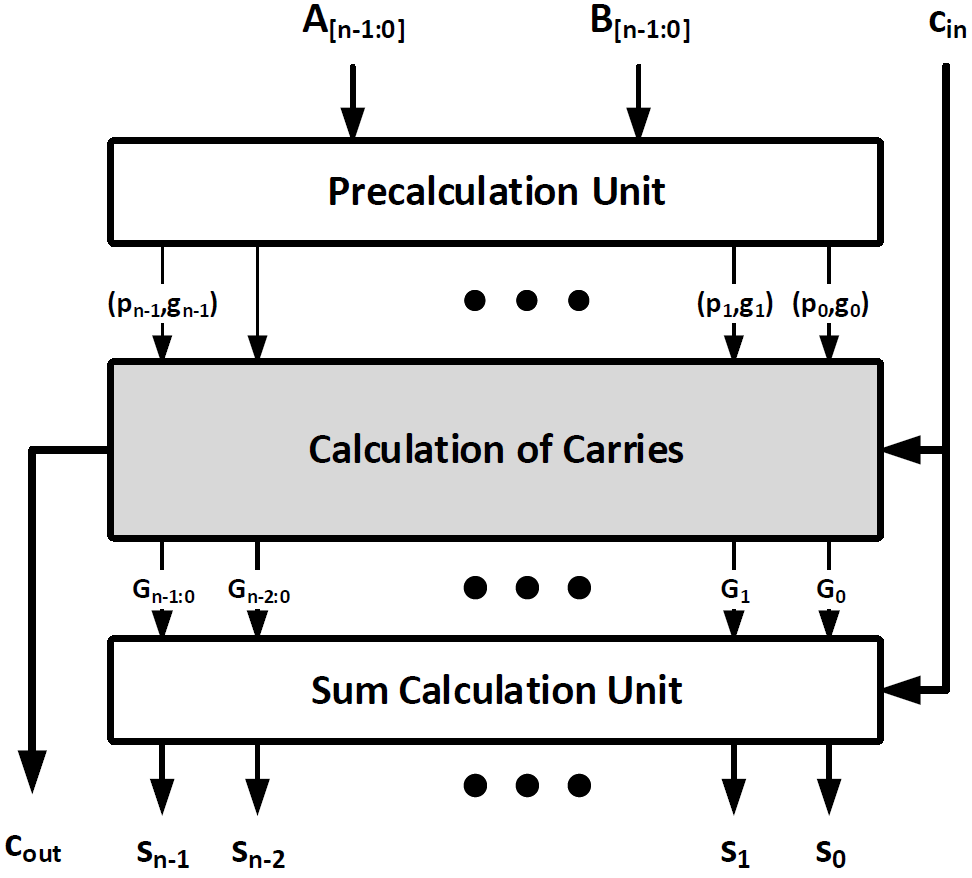
\includegraphics[height=9cm,width=10cm]{Pictures/CLA_Architecture.png}
    \caption{Αρχιτεκτονική αθροιστή πρόβλεψης κρατουμένου}
    \label{cla_architecture}
\end{figure}

Στην εικόνα \ref{cla_architecture} παρουσιάζεται η βασική αρχιτεκτονική ενός αθροιστή πρόβλεψης κρατουμένου των n δυαδικών ψηφίων. Στο πρώτο επίπεδο υπολογίζονται τα σήματα generate και propagate, στο δεύτερο τμήμα υπολογίζονται τα σήματα Group Generate (κρατούμενα $c_i$) και Group Propagate και στο τρίτο πραγματοποιείται η άθροιση. Σημειώνεται στην συγκεκριμένη αρχιτεκτονική το μεγαλύτερο λειτουργικό φόρτο καθώς και εμβαδόν καταλαμβάνει η μονάδα υπολογισμού των κρατουμένων. Στις επόμενες ενότητες θα εξεταστούν εκτενώς τεχνικές βελτιστοποίησης της μονάδας αυτής.
